\label{fig:piantaPianoTerra}
\includepdf[pages=2,pagecommand={}, angle=90, width=\textwidth]{../text/Esercitazione_01}
\label{fig:piantaPianoPrimo}
\includepdf[pages=3,pagecommand={}, angle=90, width=\textwidth]{../text/Esercitazione_01}
\label{fig:piantaPianoSecondo}
\includepdf[pages=4,pagecommand={}, angle=90, width=\textwidth]{../text/Esercitazione_01}
\label{fig:piantaCopertura}
\includepdf[pages=5,pagecommand={}, angle=90, width=\textwidth]{../text/Esercitazione_01}
\label{fig:sezione}
\includepdf[pages=6,pagecommand={}, angle=90, width=\textwidth]{../text/Esercitazione_01}

\chapter{Piante ed elementi in esame}\label{chap:piante}

Come introdotto poco sopra, si allegano gli elaborati grafici della carpenteria (pagg.~\pageref{fig:piantaPianoTerra}$\div$\pageref{fig:sezione}) forniti nel testo dell'esercitazione di Sicurezza Strutturale. Nelle seguenti righe verranno, invece, introdotti gli elemeni strutturali oggetto del dimensionamento e della verifica accompagnati dai diagrammi delle azioni interne derivati durante la suddetta esercitazione.


Secondo le indicazioni riportate nel testo, gli elementi strutturali in esame sono la trave al \emph{piano primo} che va dai pilastri $P13\div P18$ fino al \emph{vano scala}, e i pilastri $P27$ e $P36$, come segnato in figura~\ref{fig:elementiStrutturali_pianoPrimo} di pagina~\pageref{fig:elementiStrutturali_pianoPrimo}.

\section{Trave}

Come già scritto, la trave parte dal pilastro $P13$ passando per il $P18$ e si interrompe all'intersezione con il vano scala. L'elemento divide l'ambiente interno dall'ambiente esterno e ha una sezione rettangolare tale per cui non è in spessore di solaio. Ai fini del calcolo delle azioni interne, è stata considerata la sezione non armata di base $30\,cm$ e altezza $50\,cm$. 




% \begin{figure}[]
%  \centering
%  \begin{tikzpicture}[scale=.5]
%   \draw [thick, pattern=north east lines](-1.5, -2.5) rectangle (1.5, 2.5);
%   \draw [|-|] (-1.5, -3.5) -- (1.5, -3.5) node at (0, -3.5) [anchor=south]{$30\,\si{cm}$} ;
%   \draw [|-|] (-2, -2.5) -- (-2, 2.5) node at (-2, 0) [rotate=90, anchor=south]{$50\,\si{cm}$} ;
%  \end{tikzpicture}
%  \caption{Sezione della trave in cemento armato}
%  \label{fig:beamSec}
% \end{figure}

La schematizzazione della struttura ha consentito di rappresentarla come una trave continua su sette appoggi, e dunque composta da sei campate di lunghezze differenti (vedi figura~\ref{fig:schemaTrave}).

Dall'analisi dei carichi effettuata, considerando le lunghezze di influenza della trave, il valore dei carichi gravanti sull'elemento sono riportati in tabella~\ref{tab:azioniTrave}.

\begin{table}
\caption{Riepilogo dei carichi agenti sulla trave}  
\label{tab:azioniTrave}
\resizebox{\textwidth}{!}{
 \begin{tabular}{lcccccccr}
 \toprule
   &Zona\,[m]&$G_{1k}\,[kN/_{m}]$ &$G_{2k}\,[kN/_{m}]$ & $Q_{CAT. B2}\,[kN/_{m}]$&$Q_{s}\,[kN/_{m}]$&$Q_{w}\,[kN/_{m}]$\\
   \midrule
   \multirow{2}{*}{$P13\div P16$}&Interno ($\times 2.50)$&$8.00$&$11.55$&$7.50$\\
   &Esterno ($\times 3.60$) &$11.52$ &$7.98$ &$14.40$ &\begin{tabular}{c}
															$8.68$ (min)\\$15.01$ (max)
                                                       \end{tabular} &$\pm0.50$\\
	\multirow{2}{*}{$P16\div P17$}&Interno ($\times 2.50)$&$8.00$&$11.55$&$7.50$\\
   &Esterno ($\times 2.10$) &$6.72$ &$4.65$ &$8.40$ &\begin{tabular}{c}
															$5.06$ (min)\\$10.30$ (max)
                                                       \end{tabular} &$\pm0.30$\\
	\multirow{2}{*}{$P17 - VS$}&Interno ($\times 1.875)$&$6.00$&$8.66$&$5.63$\\
   &Esterno ($\times 1.00$) &$3.20$ &$2.215$ &$4.00$ &\begin{tabular}{c}
															$2.41$ (min)\\$4.17$ (max)
                                                       \end{tabular} &$\pm0.138$\\
	Trave &&$3.75$&$9.20$\\
  \bottomrule
 \end{tabular}
 }%
\end{table}

\begin{figure}
\centering
 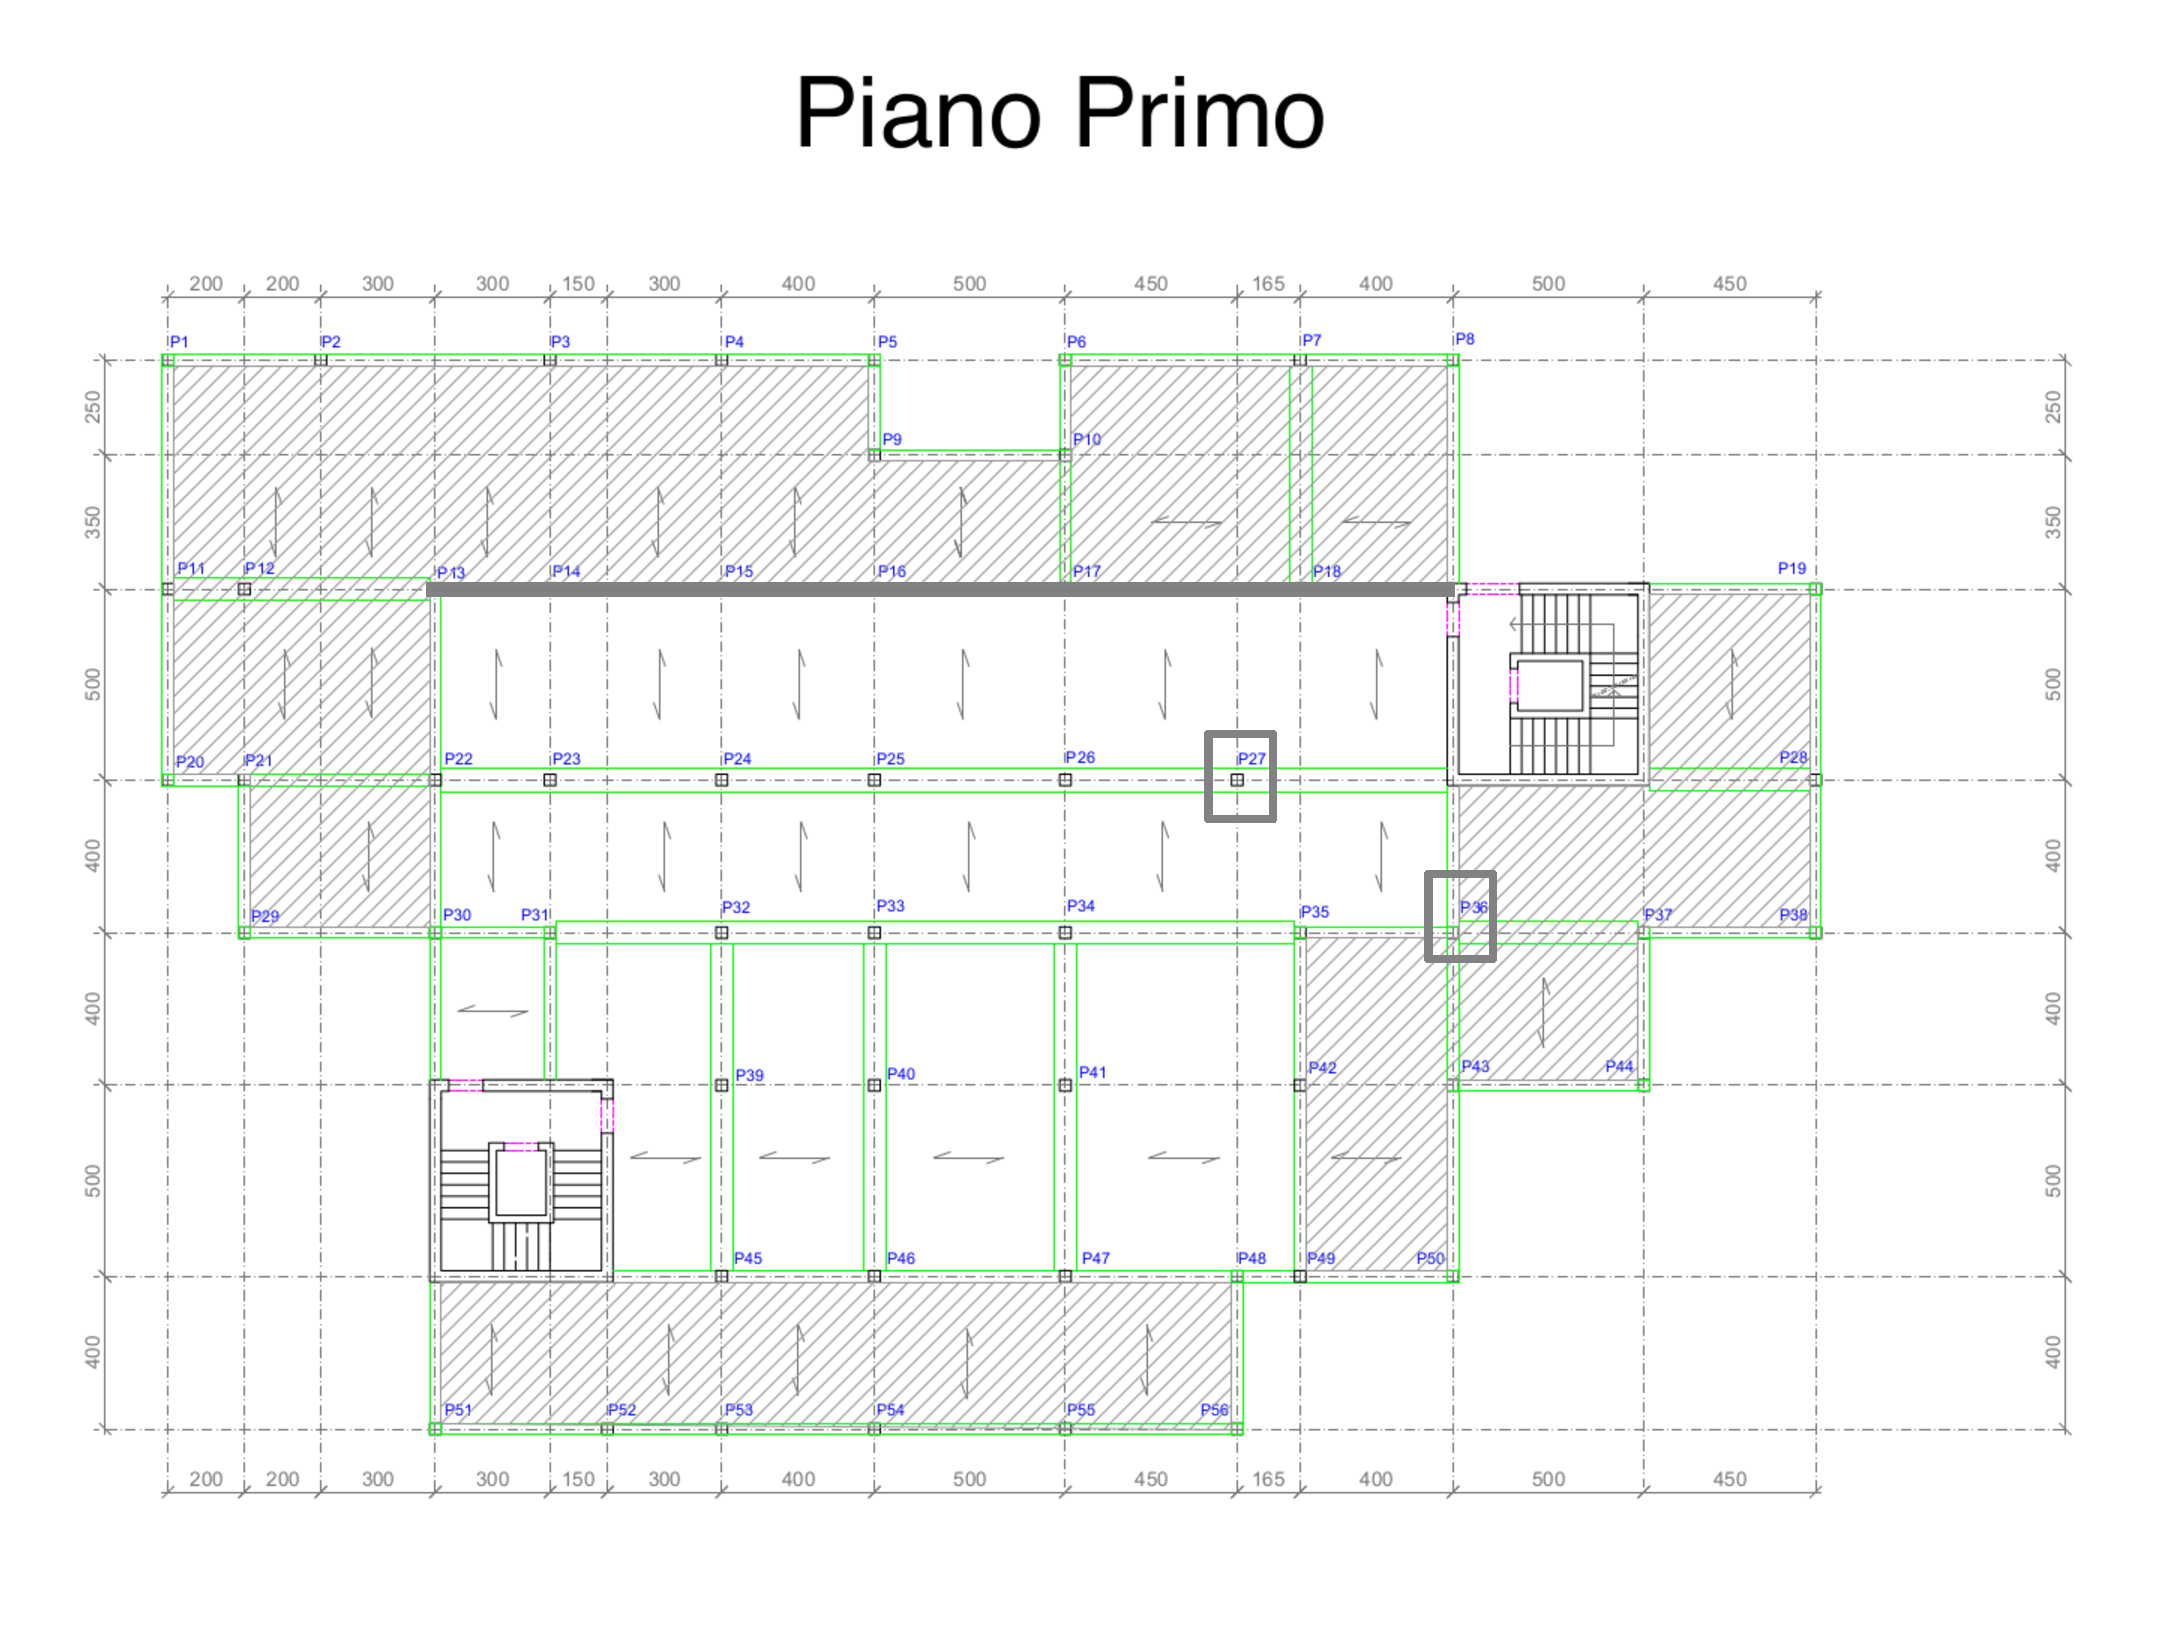
\includegraphics[width=\textwidth]{elementiStrutturali_pianoPrimo}
 \caption{Elementi strutturali oggetto di studio - piano primo}
 \label{fig:elementiStrutturali_pianoPrimo}
\end{figure}


\begin{figure}
 \centering
 \subfloat[\emph{Rappresentazione statica della trave e lunghezza delle campate}]{
 \begin{tikzpicture}
    \scaling{.45};
  \point{p13}{0}{0};
  \point{p14}{3}{0};
  \point{p15}{7.5}{0};
  \point{p16}{11.5}{0};
  \point{p17}{16.5}{0};
  \point{p18}{22.65}{0};
  \point{vs}{26.65}{0};
  
  \beam{1}{p13}{vs};
  \support{1}{p13};
  \support{2}{p14};
  \support{2}{p15};
  \support{2}{p16};
  \support{2}{p17};
  \support{2}{p18};
  \support{2}{vs};
  
  \dimensioning{1}{p13}{p14}{-1.8}[$3.00\,m$];
  \dimensioning{1}{p14}{p15}{-1.8}[$4.50\,m$];
  \dimensioning{1}{p15}{p16}{-1.8}[$4.00\,m$];
  \dimensioning{1}{p16}{p17}{-1.8}[$5.00\,m$];
  \dimensioning{1}{p17}{p18}{-1.8}[$6.15\,m$];
  \dimensioning{1}{p18}{vs}{-1.8}[$4.00\,m$];
  
  \notation{1}{p13}{$P13$};
  \notation{1}{p14}{$P14$};
  \notation{1}{p15}{$P15$};
  \notation{1}{p16}{$P16$};
  \notation{1}{p17}{$P17$};
  \notation{1}{p18}{$P18$};
  \notation{1}{vs}{$VS$};
 \end{tikzpicture}}\\
 \subfloat[\emph{Nomenclatura utilizzata per gli elementi}]{
 \begin{tikzpicture}
    \scaling{.45};
  \point{p13}{0}{0};
  \point{p14}{3}{0};
  \point{p15}{7.5}{0};
  \point{p16}{11.5}{0};
  \point{p17}{16.5}{0};
  \point{p18}{22.65}{0};
  \point{vs}{26.65}{0};
  
  \beam{1}{p13}{vs};
  \support{1}{p13};
  \support{2}{p14};
  \support{2}{p15};
  \support{2}{p16};
  \support{2}{p17};
  \support{2}{p18};
  \support{2}{vs};
  
  \notation{4}{p13}{p14}[$C1$][.7];
  \notation{4}{p14}{p15}[$C2$][.5];
  \notation{4}{p15}{p16}[$C3$][.5];
  \notation{4}{p16}{p17}[$C4$][.5];
  \notation{4}{p17}{p18}[$C5$][.5];
  \notation{4}{p18}{vs}[$C6$][.7];
  
  \notation{1}{p13}{$N1$};
  \notation{1}{p14}{$N2$};
  \notation{1}{p15}{$N3$};
  \notation{1}{p16}{$N4$};
  \notation{1}{p17}{$N5$};
  \notation{1}{p18}{$N6$};
  \notation{1}{vs}{$N7$};
 \end{tikzpicture}}
    \caption{Rappresentazione statica della trave continua}
    \label{fig:schemaTrave}
\end{figure}

\begin{figure}
	\centering
	\includegraphics[width=\textwidth]{bendingMomentComparison_slu}
	\caption{Confronto dei momenti flettenti sulle campate agli SLU}
	\label{fig:bendingMomentComparison_slu}
\end{figure}

Come si può osservare in figura~\ref{fig:schemaTrave} in via cautelativa è stato assunto, sul nodo $N7$ tra trave e vano scala, un vincolo di carrello in alternativa all'incastro. 

\noindent
Questo fa si che il momento in campata $C6$ sia maggiore ma presuppone che il nodo trave -- vano scala non sviluppi un momento flettente.

Le combinazioni delle azioni sono state effettuate secondo la normativa italiana vigente per la combinazione fondamentale agli stati limite ultimi e per le tre combinazioni agli stati limite di esercizio:
\begin{itemize}
 \item combinazione rara o caratteristica;
 \item combinazione frequente;
 \item combinazione quasi permanente.
\end{itemize}
Di seguito si riportano i diagrammi degli inviluppi delle sollecitazioni di maggior interesse (momento flettente e taglio) per gli stati limite sopra citati. 

\paragraph{Osservazione: i diagrammi dell'inviluppo (e.g. l'inviluppo dei momenti flettenti di figura~\ref{fig:bendingMomentEnvelope_slu}) sono stati ricavati dalla sovrapposizione dei diagrammi delle sollecitazioni delle otto combinazioni di carico, come dimostrato in figura~\ref{fig:bendingMomentComparison_slu}.}

\subsection{Combinazione SLU}
Per la combinazione fondamentale, gli inviluppi delle sollecitazioni sono rappresentati in figura~\ref{fig:envelope_slu}; i valori massimi e minimi delle sollecitazioni sulle sezioni di riferimento per il dimensionamento della trave sono riportati nelle tabelle~\ref{tab:bendingMoment_slu} e \ref{tab:shear_slu} di pagina~\pageref{tab:bendingMoment_slu}.

Il momento flettente massimo (in modulo) si ha in corrispondenza del nodo $N5$, con un valore di $236.63\,kN\,m$, che verrà impiegato per il primo dimensionamento della sezione. Il valore di momento minimo positivo si ha in campata $C6$, tra il pilatro $P18$ e il vano scala. Dalla figura~\ref{fig:bendingMomentEnvelope_slu} si può osservare che nelle campate centrali ($C3$ e $C4$) il momento che tende le fibre superiori non riesce ad annullarsi, il che implica che in quelle sezioni sarà necessaria una verifica specifica per quei valori di momento flettente negativo.

\begin{table}
	\centering
	\caption{Valori massimi e minimi del momento flettente in combinazione SLU}
	\label{tab:bendingMoment_slu}
    \begin{tabular*}{\textwidth}{l @{\extracolsep{\fill}} cccr}
\toprule
Sezione &  $M_{Ed}^+ [kN\,m]$ &  $s_{max} [m]$ &  $M_{Ed}^- [kN\,m]$ &  $s_{min} [m] $\\
\midrule
    C1 &    95.189448 &      1.26 &          NaN &       NaN \\
    N2 &          NaN &       NaN &  -199.249367 &      3.00 \\
    C2 &   156.565614 &      5.32 &     0.000000 &       NaN \\
    N3 &          NaN &       NaN &  -216.792778 &      7.50 \\
    C3 &   124.347537 &      9.55 &   -39.690612 &      9.47 \\
    N4 &          NaN &       NaN &  -210.348968 &     11.50 \\
    C4 &   151.829401 &     13.96 &    -6.190556 &     13.74 \\
    N5 &          NaN &       NaN &  -236.629193 &     16.50 \\
    C5 &   144.511198 &     19.56 &     0.000000 &       NaN \\
    N6 &          NaN &       NaN &  -187.959174 &     22.65 \\
    C6 &    87.580801 &     25.00 &          NaN &       NaN \\
\bottomrule
    \end{tabular*}
\end{table}

\begin{table}
	\centering
	\caption{Valori massimi e minimi del taglio in combinazione SLU}
	\label{tab:shear_slu}
    \begin{tabular*}{\textwidth}{l @{\extracolsep{\fill}} cccr}
\toprule
Sezione &   $V_{Ed}^+ [kN]$ &  $s_{max} [m]$ &   $V_{Ed}^- [kN]$ &  $s_{min} [m]$ \\
\midrule
N1 &  150.590167 &      0.00 &    0.000000 &      0.00 \\
N2 &  286.437347 &      3.00 & -245.457255 &      3.00 \\
N3 &  272.636139 &      7.50 & -286.334051 &      7.50 \\
N4 &  266.790145 &     11.50 & -266.497699 &     11.50 \\
N5 &  246.693151 &     16.50 & -261.914745 &     16.50 \\
N6 &  208.848422 &     22.65 & -202.221517 &     22.65 \\
N7 &    0.000000 &     26.65 & -105.286297 &     26.65 \\
\bottomrule
    \end{tabular*}
\end{table}

\begin{figure}
 \centering
 \subfloat[\emph{Diagramma di inviluppo dei momenti flettenti in combinazione SLU}]{
    \includegraphics[width=\textwidth]{bendingMomentEnvelope_slu}\label{fig:bendingMomentEnvelope_slu}}\\
 \subfloat[\emph{Diagramma di inviluppo dei tagli in combinazione SLU}]{ 
	 \includegraphics[width=\textwidth]{shearEnvelope_slu}\label{fig:shearEnvelope_slu}}
    
 \caption{Diagrammi degli inviluppi delle sollecitazioni per la combinazione agli SLU}
 \label{fig:envelope_slu}
\end{figure}

Per quanto riguarda il taglio, la sezione più sollecitata è in corrispondenza dell'appoggio $N2$ con un valore massimo (positivo) di $286.437\,kN$. Osservando i valori, positivi e negativi, riportati in tabella~\ref{tab:shear_slu} si può intuire che sarà sicuramente necessaria un'armatura a taglio composta da staffe in ogni appoggio.

% \cleardoublepage

\subsection{Combinazione SLE rara}

Agli stati limite di esercizio, per loro definizione, i valori delle sollecitazioni sono nettamente inferiori rispetto a quanto visto per la combinazione fondamentale. In particolare per quanto riguarda il momento flettente che, secondo quanto riportato in tebella~\ref{tab:bendingMoment_sleRara}, ha il massimo di circa $148.80\,kN\,m$ - cioè circa $2/3$ il valore del momento agli SLU in corrispondenza del medesimo nodo $N5$. Ad ogni modo, si nota che in questa combinazione delle azioni, l'inviluppo dei momenti flettenti è caratterizzato da una quasi continuità in corrispondenza dell'asse delle ascisse, che fa pensare al fatto che i diagrammi delle varie combinazioni di carico non si discostino poi di molto l'uno dall'altro. Il momento massimo di campata è di $87.16\,kN\,m$, uguagliato in $C2$.

Infine, il taglio massimo lo si raggiunge sul ramo positivo del nodo $N2$, con un valore di $186.10\,kN$.

\begin{table}[ht!]
	\centering
	\caption{Valori massimi e minimi del momento flettente in combinazione SLE rara}
	\label{tab:bendingMoment_sleRara}
    \begin{tabular*}{\textwidth}{l @{\extracolsep{\fill}} cccr}
\toprule
Sezione &  $M_{Ed}^+ [kN\,m]$ &  $s_{max} [m]$ &  $M_{Ed}^- [kN\,m]$ &  $s_{min} [m] $\\
\midrule
C1      &     44.8783 &        1 &         NaN &      NaN \\
N2      &         NaN &      NaN &     -124.53 &        3 \\
C2      &     87.1603 &     5.26 &           0 &      NaN \\
N3      &         NaN &      NaN &    -130.765 &      7.5 \\
C3      &     49.5098 &     9.52 &           0 &      NaN \\
N4      &         NaN &      NaN &    -121.154 &     11.5 \\
C4      &     76.7491 &     13.9 &           0 &      NaN \\
N5      &         NaN &      NaN &    -148.799 &     16.5 \\
C5      &     79.7629 &     19.7 &           0 &      NaN \\
N6      &         NaN &      NaN &    -117.967 &    22.65 \\
C6      &     41.9934 &       25 &         NaN &      NaN \\
\bottomrule
    \end{tabular*}
\end{table}

\begin{table}[ht!]
	\centering
	\caption{Valori massimi e minimi del taglio in combinazione SLE rara}
	\label{tab:shear_sleRara}
    \begin{tabular*}{\textwidth}{l @{\extracolsep{\fill}} cccr}
\toprule
Sezione &  $V_{Ed}^+ [kN]$ &  $s_{max} [m]$ &  $V_{Ed}^- [kN]$ &  $s_{min} [m] $\\
\midrule
N1      &   83.9204 &        0 &         0 &        0 \\
N2      &   186.094 &        3 &  -165.135 &        3 \\
N3      &   169.265 &      7.5 &  -188.299 &      7.5 \\
N4      &   158.119 &     11.5 &  -165.893 &     11.5 \\
N5      &   140.929 &     16.5 &  -170.792 &     16.5 \\
N6      &   116.471 &    22.65 &  -131.627 &    22.65 \\
N7      &         0 &    26.65 &  -59.6292 &    26.65 \\
\bottomrule
    \end{tabular*}
\end{table}




\begin{figure}
 \centering
 \subfloat[\emph{Diagramma di inviluppo dei momenti flettenti in combinazione SLE rara}]{
    \includegraphics[width=\textwidth]{bendingMomentEnvelope_sleRara}\label{fig:bendingMomentEnvelope_sleRara}}\\
 \subfloat[\emph{Diagramma di inviluppo dei tagli in combinazione SLE rara}]{ 
    \includegraphics[width=\textwidth]{shearEnvelope_sleRara}
    \label{fig:shearEnvelope_sleRara}}
    
 \caption{Diagrammi degli inviluppi delle sollecitazioni per la combinazione agli SLE rara}
 \label{fig:envelope_sleRara}
\end{figure}

%-----------------------------------------------------------
\cleardoublepage
\subsection{Combinazione SLE frequente}

Di seguito si riportano le tabelle e i diagrammi delle sollecitazioni per quanto riguarda la combinazione agli SLE frequente.

\begin{table}[ht!]
	\centering
	\caption{Valori massimi e minimi del momento flettente in combinazione SLE frequente}
	\label{tab:bendingMoment_sleFreq}
    \begin{tabular*}{\textwidth}{l @{\extracolsep{\fill}} cccr}
\toprule
Sezione &  $M_{Ed}^+ [kN\,m]$ &  $s_{max} [m]$ &  $M_{Ed}^- [kN\,m]$ &  $s_{min} [m] $\\
\midrule
C1      &     31.3072 &        1 &         NaN &      NaN \\
N2      &         NaN &      NaN &    -91.5441 &        3 \\
C2      &     62.6374 &     5.26 &           0 &      NaN \\
N3      &         NaN &      NaN &    -95.1011 &      7.5 \\
C3      &     32.4615 &     9.52 &           0 &      NaN \\
N4      &         NaN &      NaN &    -88.3851 &     11.5 \\
C4      &     55.1968 &    13.87 &           0 &      NaN \\
N5      &         NaN &      NaN &    -119.521 &     16.5 \\
C5      &     65.9368 &     19.7 &           0 &      NaN \\
N6      &         NaN &      NaN &    -98.8067 &    22.65 \\
C6      &     33.2037 &       25 &         NaN &      NaN \\
\bottomrule
    \end{tabular*}
\end{table}

\begin{table}[ht!]
	\centering
	\caption{Valori massimi e minimi del taglio in combinazione SLE frequente}
	\label{tab:shear_sleFreq}
    \begin{tabular*}{\textwidth}{l @{\extracolsep{\fill}} cccr}
\toprule
Sezione &  $V_{Ed}^+ [kN]$ &  $s_{max} [m]$ &  $V_{Ed}^- [kN]$ &  $s_{min} [m] $\\
\midrule
N1      &   147.527 &        0 &         0 &        0 \\
N2      &   284.831 &        3 &      -244 &        3 \\
N3      &   270.033 &      7.5 &  -285.874 &      7.5 \\
N4      &    249.12 &     11.5 &  -266.217 &     11.5 \\
N5      &   211.204 &     16.5 &  -260.609 &     16.5 \\
N6      &    172.32 &    22.65 &   -202.19 &    22.65 \\
N7      &         0 &    26.65 &  -103.721 &    26.65 \\
\bottomrule
    \end{tabular*}
\end{table}




\begin{figure}
 \centering
 \subfloat[\emph{Diagramma di inviluppo dei momenti flettenti in combinazione SLE frequente}]{
    \includegraphics[width=\textwidth]{bendingMomentEnvelope_sleFreq}\label{fig:bendingMomentEnvelope_sleFreq}}\\
 \subfloat[\emph{Diagramma di inviluppo dei tagli in combinazione SLE frequente}]{ 
    \includegraphics[width=\textwidth]{shearEnvelope_sleFreq}
    \label{fig:shearEnvelope_sleFreq}}
    
 \caption{Diagrammi degli inviluppi delle sollecitazioni per la combinazione agli SLE frequente}
 \label{fig:envelope_sleFreq}
\end{figure}

%-----------------------------------------------------------
\cleardoublepage
\subsection{Combinazione SLE quasi permanente}

L'ultima combinazione delle azioni richieste dalla normativa italiana è la combinazione quasi permanente. Come fatto in precedenza, si allegano i valori delle sollecitazioni sulle sezioni di riferimento e i diagrammi delle azioni interne.

\begin{table}[ht!]
	\centering
	\caption{Valori massimi e minimi del momento flettente in combinazione SLE quasi permanente}
	\label{tab:bendingMoment_sleQP}
    \begin{tabular*}{\textwidth}{l @{\extracolsep{\fill}} cccr}
\toprule
Sezione &  $M_{Ed}^+ [kN\,m]$ &  $s_{max} [m]$ &  $M_{Ed}^- [kN\,m]$ &  $s_{min} [m] $\\
\midrule
C1      &     29.1805 &        1 &         NaN &      NaN \\
N2      &         NaN &      NaN &    -86.7303 &        3 \\
C2      &     58.9209 &     5.23 &           0 &      NaN \\
N3      &         NaN &      NaN &    -89.9972 &      7.5 \\
C3      &     29.8967 &     9.52 &           0 &      NaN \\
N4      &         NaN &      NaN &    -83.7524 &     11.5 \\
C4      &     52.1556 &    13.87 &           0 &      NaN \\
N5      &         NaN &      NaN &    -115.072 &     16.5 \\
C5      &     63.7428 &     19.7 &           0 &      NaN \\
N6      &         NaN &      NaN &    -95.7222 &    22.65 \\
C6      &     31.8861 &    25.32 &         NaN &      NaN \\
\bottomrule
    \end{tabular*}
\end{table}

\begin{table}[ht!]
	\centering
	\caption{Valori massimi e minimi del taglio in combinazione SLE quasi permanente}
	\label{tab:shear_sleQP}
    \begin{tabular*}{\textwidth}{l @{\extracolsep{\fill}} cccr}
\toprule
Sezione &  $V_{Ed}^+ [kN]$ &  $s_{max} [m]$ &  $V_{Ed}^- [kN]$ &  $s_{min} [m] $\\
\midrule
N1      &   83.9204 &        0 &         0 &        0 \\
N2      &   186.094 &        3 &  -165.135 &        3 \\
N3      &   169.265 &      7.5 &  -188.299 &      7.5 \\
N4      &   158.119 &     11.5 &  -165.893 &     11.5 \\
N5      &   140.929 &     16.5 &  -170.792 &     16.5 \\
N6      &   116.471 &    22.65 &  -131.627 &    22.65 \\
N7      &         0 &    26.65 &  -59.6292 &    26.65 \\
\bottomrule
    \end{tabular*}
\end{table}




\begin{figure}
 \centering
 \subfloat[\emph{Diagramma di inviluppo dei momenti flettenti in combinazione SLE quasi permanente}]{
    \includegraphics[width=\textwidth]{bendingMomentEnvelope_sleQP}\label{fig:bendingMomentEnvelope_sleQP}}\\
 \subfloat[\emph{Diagramma di inviluppo dei tagli in combinazione SLE quasi permanente}]{ 
    \includegraphics[width=\textwidth]{shearEnvelope_sleQP}
    \label{fig:shearEnvelope_sleQP}}
 \caption{Diagrammi degli inviluppi delle sollecitazioni per la combinazione agli SLE quasi permanente}
 \label{fig:envelope_sleQP}
\end{figure}

%---------------------------------------------
\cleardoublepage

\section{Solaio}\label{sec:azioniSolaio}

\begin{figure}
	\centering
	\includegraphics[height=\textwidth, angle=-90]{solaioPianoSecondo}
	\caption{Scelta del solaio da progettare e verificare}
	\label{fig:solaioPianoSecondo}
\end{figure}

Il solaio da analizzare è stato scelto in modo tale che fosse un solaio in laterocemento (solai interni), a due campate e, per evitare ripetitività e ridondanze, che non fosse posto allo stesso livello della trave. Per questo si è optato per il solaio al piano secondo rappresentato in figura~\ref{fig:solaioPianoSecondo}. Per ovviare a condizioni di particolare simmetria dei carichi e quindi delle azioni interne, si è preferito scegliere il solaio continuo tra due campate di luce differente: l'orditura del solaio infatti prevede una campata di $4.00\,m$ e una campata di $5.00\,m$.

\begin{figure}
 \centering
 \subfloat[\emph{Rappresentazione statica del solaio e lunghezza delle campate}]{
 \begin{tikzpicture}
    \scaling{1};
  \point{p33}{0}{0};
  \point{p40}{4}{0};
  \point{p46}{9}{0};

  
  \beam{1}{p33}{p46};
  \support{1}{p33};
  \support{2}{p40};
  \support{2}{p46};
  
  \dimensioning{1}{p33}{p40}{-1.8}[$4.00\,m$];
  \dimensioning{1}{p40}{p46}{-1.8}[$5.00\,m$];

  \notation{1}{p33}{$P33$};
  \notation{1}{p40}{$P40$};
  \notation{1}{p46}{$P46$};
 \end{tikzpicture}}\\
 \subfloat[\emph{Nomenclatura utilizzata per gli elementi}]{
 \begin{tikzpicture}
    \scaling{1};
  \point{p33}{0}{0};
  \point{p40}{4}{0};
  \point{p46}{9}{0};

  
  \beam{1}{p33}{p46};
  \support{1}{p33};
  \support{2}{p40};
  \support{2}{p46};
  
  \notation{4}{p33}{p40}[$CS1$];
  \notation{4}{p40}{p46}[$CS2$];
  
  \notation{1}{p33}{$NS1$};
  \notation{1}{p40}{$NS2$};
  \notation{1}{p46}{$NS3$};
  
    \dimensioning{1}{p33}{p40}{-1.8}[$l_1$];
  \dimensioning{1}{p40}{p46}{-1.8}[$l_2$];

 \end{tikzpicture}}
    \caption{Rappresentazione statica del solaio continuo a due campate}
    \label{fig:schemaSolaio}
\end{figure}

Procedendo allo stesso modo per quanto fatto per la trave, si risolve la struttura con il metodo delle forze - andando a inserire delle cerniere interne in corrispondenza degli appoggi interni (dove è presente continuità) e applicando il relativo momento concentrato al nodo.

\begin{figure}[t]
	\centering
	\begin{tikzpicture}
    \scaling{1};
  \point{p33}{0}{0};
  \point{p40}{4}{0};
  \point{p46}{9}{0};

  
  \beam{1}{p33}{p46};
  \support{1}{p33};
  \support{2}{p40};
  \support{2}{p46};
  
  \hinge{1}{p33};
  \hinge{1}{p40};
  \hinge{1}{p46};
%   \notation{4}{p33}{p40}[$CS1$];
%   \notation{4}{p40}{p46}[$CS2$];
%   
%   \notation{1}{p33}{$NS1$};
%   \notation{1}{p40}{$NS2$};
%   \notation{1}{p46}{$NS3$};
  
  \load{2}{p40}[100][130][1];
  \load{3}{p40}[130][130][-1];
  
  \notation{1}{p40}{$m_2$}[above=10mm];

    \lineload{1}{p33}{p40}[.8][.8];
    \lineload{1}{p40}{p46}[.5][.5];
    
    \notation{1}{p33}{$q_1$}[above right=20mm];
    \notation{1}{p46}{$q_2$}[above left=15mm];

 \end{tikzpicture}
    \caption{Soluzione statica della trave continua -- metodo delle forze}
    \label{fig:staticSolution}
\end{figure}

Applicando la condizione di compatibilità sulle rotazioni al nodo centrale ($NS2$) ci si riconduce alla forma matriciale generica
\[
	\doubleunderline{K}\cdot \underline{X} = \underline{F}
\]
dove $\doubleunderline{K}$ è la matrice di rigidezza della struttura, $\underline{X}$ è il vettore dei momenti incogniti ai nodi e $\underline{F}$ è il vettore dei carichi esterni applicati.  
In questo particolare caso, avendo svincolato un solo nodo, il sistema si riconduce a un'unica equazione scalare
\[
	\dfrac{2\,l_1 + 2\,l_2}{6\,EJ} \cdot m_2 = -\dfrac{q_1\,l_1^3 + q_2\,l_2^3}{24\,EJ}
\]

\begin{figure}[ht!]
	\centering
	\subfloat[\emph{Diagramma del momento flettente con carico unitario applicato sulla prima campata}]{
	\includegraphics[width=\textwidth]{../../export/img/bendingMoment_loadSpan_1}}\\
	\subfloat[\emph{Diagramma del momento flettente con carico unitario applicato sulla seconda campata}]{
	\includegraphics[width=\textwidth]{../../export/img/bendingMoment_loadSpan_2}}
	\caption{Diagramma dei momenti flettenti per carichi distribuiti unitari sulle campate}
	\label{fig:loadOnSpan}
\end{figure}

A questo punto il sistema sarebbe staticamente determinato se fossero noti i carichi $q_1$ e $q_2$. In prima approssimazione si può risolvere il sistema ponendo prima il carico $q_1$ pari all'unità (e $q_2 = 0$) e poi il suo duale $q_1 = 0$, $q_2 = 1$. In entrambi i casi, una volta ottenute le reazioni vincolari, si ricava l'andamento del diagramma del momento flettente per il carico unitario considerato; quello che ne consegue è rappresentato in figura~\ref{fig:loadOnSpan}. I diagrammi rappresentati vanno confrontati con il generico diagramma del momento flettente di una trave continua a due campate, da cui si deducono le combinazioni di carico significative, che in questo caso sono tre:
\begin{itemize}
	\item combinazione \texttt{MAX-MIN};
	\item combinazione \texttt{MAX-MAX};
	\item combinazione \texttt{MIN-MAX}.
\end{itemize}

\paragraph{Osservazione: è stato applicato il medesimo procedimento anche per gli sforzi di taglio ma, per una questione di ripetitività, si è deciso di non riportare i passaggi.}

\subsection{Analisi dei carichi}
Il solaio oggetto di studio è situato al secondo piano, in cui è prevista una destinazione d'uso di civile abitazione. Nelle righe che seguono verranno calcolati i carichi distribuiti gravanti su un metro quadro di solaio.

\subsubsection*{Carichi permanenti strutturali}
Nei carichi permanenti strutturali ricade il peso proprio del solaio che è stato definito nel capitolo~\ref{chap:intro}.

\[
	g_{1k} = 3.20\,\dfrac{kN}{m^2}
\]

\subsubsection*{Carichi permanenti non strutturali}
Essendo un solaio interno, il contributo dei carichi permanenti non strutturali è dato da

\begin{align*}
 g_{2k, sottofondo} &= \gamma_{cls, all}\cdot s_{sottofondo} = 16\,\dfrac{kN}{m^3}\cdot 0.08\,\si{m} = 1.28\,\dfrac{kN}{m^2}\\
 g_{2k, massetto} &= \gamma_{massetto}\cdot
 s_{massetto} = 24\,\dfrac{kN}{m^3}\cdot 0.06\,\si{m} = 1.44\,\dfrac{kN}{m^2}\\
 g_{2k, pavimento} &= 0.50\,\dfrac{kN}{m^2}\\
 g_{2k, intonaco} &= \gamma_{intonaco}\cdot s_{intonaco} = 20\,\dfrac{kN}{m^3}\cdot 0.01\,\si{m} = 0.20\,\dfrac{kN}{m^2}
\end{align*}

Inoltre, il carico lineare dato dalle tramezze interne può essere calcolato come segue

\begin{align*}
 G_{2, div} &= \gamma_{div} \cdot s_{div} \cdot h_{div} + 2 \cdot \gamma_{intonaco} \cdot s_{intonaco} \cdot h_{div} =\\ &= 8.00\,\dfrac{kN}{m^3}\cdot 0.08\,\si{m} \cdot (3.10 - 0.25)\,\si{m} + 20\,\dfrac{kN}{m^3}\cdot 0.01\,\si{m} \cdot (3.10 - 0.25 - 0.01)\,\si{m}=\\ &= 2.96\,\dfrac{kN}{m}
\end{align*}
 
La normativa consente di convertire il carico per unità di lunghezza  delle divisorie in un carico uniformemente distribuito su un'area. Per elementi divisori con $2<G_2 \leq 3\,kN/_m$ si ha
\[
    g_{2k, div} = 1.20\,\dfrac{kN}{m^2}
\]

In definitiva i carichi permanenti non strutturali agenti sul solaio valgono
\begin{align*}
    g_{2k} &= g_{2k, sottofondo} + g_{2k, massetto} + g_{2k, pavimento} + g_{2k, intonaco} + g_{2k, div}=\\ &= (1.28 + 1.44 + 0.50 + 0.20 + 1.20)\,\dfrac{kN}{m^2} =\\&=
    4.62\,\dfrac{kN}{m^2}
\end{align*}

\subsubsection*{Carichi variabili}
Come specificato poco sopra, la destinazione d'uso dell'ambiente è di civile abitazione; nel capitolo~$3.1.4$ delle $NTC2018$ riferito ai sovraccarichi è presente la Tab.~$3.1.II$-\textit{Valori dei sovraccarichi per la diverse categorie d'uso delle costruzioni}, da cui si ricava il valore del carico variabile ricadente nella categoria $A$-\textit{Ambienti ad uso residenziale}, che vale

\[
	q_k = 2\,\dfrac{kN}{m^2}
\]
% 
\subsection{Combinazione delle azioni}
Nel caso del solaio, la combinazione delle azioni interne di riferimento sono quelle agli \textit{Stati Limite Ultimi}. Le \textit{Norme Tecniche per le Costruzioni 2018} nel capitolo $2.5.3$ definiscono la combinazione fondamentale come segue:
\[
	\gamma_{G1}\cdot G_{1k} + \gamma_{G2}\cdot G_{2k} + \gamma_{Q1} \cdot Q_{1k} + \gamma_{Q2}\cdot \psi_{02}\cdot Q_{2k} + \gamma_{Q3}\cdot \psi_{03}\cdot Q_{3k} + \dots
\]

Essendo presente un solo carico variabile, la combinazione delle azioni è facilmente calcolata. I coefficienti di combinazione sono stati estrapolati dalla Tab.~$2.5.I$ delle \textit{Norme Tecniche per le Costruzioni} del 2018 e sono riportati in tabella~\ref{tab:coeffAzioni}.

\begin{table}[ht!]
	\centering
	\caption{Valori dei coefficienti di combinazione}
	\label{tab:coeffAzioni}
    \begin{tabular*}{\textwidth}{l @{\extracolsep{\fill}} ccccr}
\toprule
&$\gamma_{\MakeUppercase{sf}}$ & $\gamma_{\MakeUppercase{f}}$ &$\psi_{0i}$ &$\psi_{1i}$ &$\psi_{2i}$\\
\midrule
$G_1$ & $1.3$ &$1.0$\\
$G_2$ &$1.5$ &$0.8$\\
$Q_{CAT. A}$ &$1.5$ &$0$ &$0.7$ &$0.5$ &$0.3$\\
\bottomrule
    \end{tabular*}
\end{table}

Allora, i valori del carico massimo e minimo distribuito sul solaio sono

\begin{align*}
	q_{max} &= \gamma_{G1,SF}\,g_{1k} + \gamma_{G2,SF}\,g_{2k} + \gamma_{Q,SF}\,q_{k} =\\
	&= 1.3\cdot 3.2 + 1.5\cdot 4.62 + 1.5\cdot 2 = 14.10\,\dfrac{kN}{m^2}
\end{align*}
\begin{align*}
	q_{min} &= \gamma_{G1,F}\,g_{1k} + \gamma_{G2,F}\,g_{2k} + \gamma_{Q,F}\,q_{k} =\\
	&= 1.0\cdot 3.2 + 0.8\cdot 4.62 + 0\cdot 2 = 6.90\,\dfrac{kN}{m^2}
\end{align*}

Come si può notare, questi valori sono riferiti ad un carico distribuito su un'area. Supponendo di considerare una striscia di solaio di $1\,m$, i carichi distribuiti su una linea risultano

\begin{align*}
	Q_{max} &= 14.10\,\dfrac{kN}{m^2}\cdot 1\,m = 14.10\,\dfrac{kN}{m}\\
	Q_{min} &= 6.90\,\dfrac{kN}{m^2}\cdot 1\,m = 6.90\,\dfrac{kN}{m}
\end{align*}

\subsubsection*{Momento flettente}

I valori appena trovati vanno moltiplicati per l'andamento dei momenti calcolato in precedenza in modo tale da definire le combinazioni di carico; ad esempio, per la prima combinazione ($MAX-MIN$)
\[
	Q_{max}\cdot M_1(s) + Q_{min}\cdot M_2(s)
\]
da cui si ricava la curva $M_{C1}$ di figura~\ref{fig:bendingMomentComparison_solaio}

\begin{figure}
	\centering
	\includegraphics[width=\textwidth]{../../export/img/bendingMomentComparison_slu}
	\caption{Confronto delle tre combinazioni di carico: $MAX-MIN$, $MAX-MAX$, $MIN-MAX$}
    \label{fig:bendingMomentComparison_solaio}
\end{figure}

Si procede analogamente e si trovano le curve $M_{N2}$ e $M_{C2}$.

L'inviluppo dei momenti flettenti ricavato è quello di figura~\ref{fig:bendingMomentEnvelope_solaio} di pagina~\pageref{fig:bendingMomentEnvelope_solaio}.

\begin{figure}
	\centering
	\includegraphics[width=\textwidth]{../../export/img/bendingMomentEnvelopeSolaio_slu}
	\caption{Inviluppo dei momenti flettenti del solaio}
	\label{fig:bendingMomentEnvelope_solaio}
\end{figure}

I valori significativi sono riportati nella seguente tabella.

\begin{table}[ht!]
	\centering
	\caption{Valori massimi e minimi del momento flettente su $1\,m$ di solaio}
	\label{tab:bendingMoment_solaio}
    \begin{tabular*}{\textwidth}{l @{\extracolsep{\fill}} cccr}
\toprule
Sezione &  $M_{Ed}^+ [kN\,m]$ &  $s_{max} [m]$ &  $M_{Ed}^- [kN\,m]$ &  $s_{min} [m] $\\
\midrule
CS1      &     30.0855 &     2.07 &         NaN &      NaN \\
NS2      &         NaN &      NaN &    -36.9699 &        5 \\
CS2      &     17.2754 &     7.44 &           0 &      NaN \\
\bottomrule
    \end{tabular*}
\end{table}

\subsubsection*{Taglio}

Il procedimento deve essere applicato anche per il taglio e fornisce il diagramma di inviluppo di figura~\ref{fig:shearEnvelope_solaio} e la tabella~\ref{tab:shear_solaio} dei valori significativi del taglio.

\begin{table}[ht!]
	\centering
	\caption{Valori massimi e minimi del taglio su $1\,m$ di solaio}
	\label{tab:shear_solaio}
    \begin{tabular*}{\textwidth}{l @{\extracolsep{\fill}} cccr}
\toprule
Sezione &  $V_{Ed}^+ [kN]$ &  $s_{max} [m]$ &  $V_{Ed}^- [kN]$ &  $s_{min} [m] $\\
\midrule
NS1      &   29.1134 &        0 &         0 &        0 \\
NS2      &    37.439 &        5 &  -42.6525 &        5 \\
NS3      &  0 &        9 &  -22.0437 &        9 \\
\bottomrule
    \end{tabular*}
\end{table}

\begin{figure}
	\centering
	\includegraphics[width=\textwidth]{../../export/img/shearEnvelopeSolaio_slu}
	\caption{Inviluppo dei tagli del solaio}
	\label{fig:shearEnvelope_solaio}
\end{figure}

%----------------------------------------------------------------------------------
\cleardoublepage
\section{Pilastri}\label{sec:azioniPilastri}

Come riportato in figura~\ref{fig:elementiStrutturali_pianoPrimo} di pagina~\pageref{fig:elementiStrutturali_pianoPrimo} i pilastri analizzati durante il corso di Sicurezza Strutturale sono i $P27$ e $P36$. Il primo è un pilastro centrale, mentre il secondo è un pilastro d'angolo che divide l'ambiente interno dall'ambiente esterno. Al piano primo, il pilastro $P36$ divide l'area interna di destinazione ad uffici aperti al pubblico dal terrazzo esterno.

L'analisi delle caratteristiche di sollecitazione sui pilastri è stata eseguita rimuovendo l'ipotesi di presso-flessione e postulando, perciò, la presenza di soli sforzi di compressione. Dai calcoli effettuati sono stati ricavati i diagrammi della sollecitazione di azione assiale massima e minima agente sui pilastri, per ogni stato limite definito dalla normativa tecnica.

\subsection{Pilastro $P27$}

\subsubsection{Combinazione agli SLU}

Dalla combinazione agli stati limite ultimi si ricavano i diagrammi di figura~\ref{fig:P27_axialLoad_slu}.

\begin{figure}
    \centering
	\subfloat[\emph{Azione assiale massima agente sul pilastro $P27$ in combinazione SLU}]{
		\includegraphics[width=\textwidth]{P27_maxAxialLoad_slu}}\\
	\subfloat[\emph{Azione assiale minima agente sul pilastro $P27$ in combinazione SLU}]{
		\includegraphics[width=\textwidth]{P27_minAxialLoad_slu}}
	\caption{Diagramma dell'azione assiale in combinazione SLU sul pilastro $P27$}
	\label{fig:P27_axialLoad_slu}
\end{figure}

\begin{table}
    \centering
	\caption{Valori massimi e minimi dell'azione assiale di compressione sul pilastro $P27$ in combinazione SLU}
	\label{tab:P27_axialLoad_slu}
	\begin{tabular*}{\textwidth}{l @{\extracolsep{\fill}} cr}
		\toprule
		$s\,[m]$ & $N_{max}\,[kN]$ & $N_{min}\,[kN]$ \\
		\midrule
		0.00 &   385.05600 &   180.8920 \\
		2.85 &   393.39225 &   187.3045 \\
		5.95 &   854.78775 &   431.0467 \\
		9.45 &  1361.77705 &   678.8797 \\
		12.20 &  1881.88080 &   886.7112 \\
		\bottomrule
	\end{tabular*}
\end{table}

Come introdotto nel capitolo~\ref{chap:intro}, i pilastro $P27$ ha sezione iniziale, in prima approssimazione, di dimensioni $30\times30\,cm$. Di seguito si riportano i diagrammi per le varie combinazioni delle azioni.
\noindent
I valori massimi di compressione ad ogni livello sono riportati in tabella~\ref{tab:P27_axialLoad_slu}

Si riscontra che l'azione massima calcolata per la combinazione fondamentale è in prossimità della base del pilastro e vale circa $1882\,kN$. Considerando invece, per il calcolo dell'azione minima, i coefficienti di sicurezza favorevoli, il valore alla base è di circa $887\,kN$.

\subsubsection{Combinazione agli SLE rara}

\begin{figure}
	\centering
	\subfloat[\emph{Azione assiale massima agente sul pilastro $P27$ in combinazione SLE rara}]{
		\includegraphics[width=\textwidth]{P27_maxAxialLoad_sleRara}}\\
	\subfloat[\emph{Azione assiale minima agente sul pilastro $P27$ in combinazione SLE rara}]{
		\includegraphics[width=\textwidth]{P27_minAxialLoad_sleRara}}
	\caption{Diagramma dell'azione assiale in combinazione SLE rara sul pilastro $P27$}
	\label{fig:P27_axialLoad_sleRara}
\end{figure}

\begin{table}
	\centering
	\caption{Valori massimi e minimi dell'azione assiale di compressione sul pilastro $P27$ in combinazione SLE rara}
	\label{tab:P27_axialLoad_sleRara}
	\begin{tabular*}{\textwidth}{l @{\extracolsep{\fill}} cr}
		\toprule
		$s\,[m]$ & $N_{max}\,[kN]$ & $N_{min}\,[kN]$ \\
		\midrule
		0.00 &   273.0600 &   232.8400 \\
		2.85 &   279.4725 &   239.2525 \\
		5.95 &   605.6715 &   565.4515 \\
		9.45 &   961.0725 &   937.7725 \\
		12.20 &  1321.9000 &  1281.6800 \\
		\bottomrule
	\end{tabular*}
\end{table}

Dalla combinazione caratteristica si ricavano la figura~\ref{fig:P27_axialLoad_sleRara} e la tabella~\ref{tab:P27_axialLoad_sleRara}. Il massimo alla base vale circa $1322\,kN$ mentre il minimo valore alla base è di circa $1282\,kN$

\subsubsection{Combinazione agli SLE frequente}

\begin{figure}
	\centering
	\subfloat[\emph{Azione assiale massima agente sul pilastro $P27$ in combinazione SLE frequente}]{
		\includegraphics[width=\textwidth]{P27_maxAxialLoad_sleFreq}}\\
	\subfloat[\emph{Azione assiale minima agente sul pilastro $P27$ in combinazione SLE frequente}]{
		\includegraphics[width=\textwidth]{P27_minAxialLoad_sleFreq}}
	\caption{Diagramma dell'azione assiale in combinazione SLE frequente sul pilastro $P27$}
	\label{fig:P27_axialLoad_sleFreq}
\end{figure}

\begin{table}
	\centering
	\caption{Valori massimi e minimi dell'azione assiale di compressione sul pilastro $P27$ in combinazione SLE frequente}
	\label{tab:P27_axialLoad_sleFreq}
	\begin{tabular*}{\textwidth}{l @{\extracolsep{\fill}} cr}
		\toprule
		$s\,[m]$ & $N_{max}\,[kN]$ & $N_{min}\,[kN]$ \\
		\midrule
		0.00 &   216.3520 &   201.9800 \\
		2.85 &   222.7645 &   208.3925 \\
		5.95 &   520.7635 &   495.1115 \\
		9.45 &   845.4995 &   800.8135 \\
		12.20 &  1156.2450 &  1100.5050 \\
		\bottomrule
	\end{tabular*}
\end{table}

La combinazione delle azioni interne agli SLE frequente genera la figura~\ref{fig:P27_axialLoad_sleFreq} e la tabella~\ref{tab:P27_axialLoad_sleFreq}. La massima e la minima azione di compressione alla base del pilastro valgono rispettivamente $1156\,kN$ e $1101\,kN$.

\subsubsection{Combinazione agli SLE quasi permanente}

\begin{figure}
	\centering
	\includegraphics[width=\textwidth]{P27_axialLoad_sleQP}
	\caption{Diagramma dell'azione assiale in combinazione SLE quasi permanente sul pilastro $P27$}
	\label{fig:P27_axialLoad_sleQP}
\end{figure}

\begin{table}
	\centering
	\caption{Valori dell'azione assiale di compressione sul pilastro $P27$ in combinazione SLE quasi permanente}
	\label{tab:P27_axialLoad_sleQP}
	\begin{tabular*}{.6 \textwidth}{l @{\extracolsep{\fill}} r}
		\toprule
		$s\,[m]$ & $N\,[kN]$\\
		\midrule
		0.00 &   202.7600 \\
		2.85 &   209.1725 \\
		5.95 &   495.8915 \\
		9.45 &   801.5935 \\
		12.20 &  1101.2850 \\
		\bottomrule
	\end{tabular*}
\end{table}

Gli SLE quasi permanente hanno un'unica combinazione delle azioni interne, il cui diagramma è rappresentato in figura~\ref{fig:P27_axialLoad_sleQP}. I valori notevoli sono riportati in tabella~\ref{tab:P27_axialLoad_sleQP}. Il valore di maggior interesse è quello alla base che risulta essere di $1101\,kN$.
\cleardoublepage
%
%
%-------------------------------------------
%
%
\subsection{Pilastro $P36$}
Come già introdotto sopra, il pilastro $P36$ è un pilastro d'angolo che divide, al piano primo, l'ambiente interno dal terrazzo. Nonostante ciò, le sollecitazioni assiali risultano di minor rilevanza rispetto al pilastro centrale.

Di seguito si riportano i diagrammi di azione assiale (di compressione) per le varie configurazioni di carichi.
\subsubsection{Combinazione agli SLU}
Dalla combinazione agli stati limite ultimi si ricavano i diagrammi di figura~\ref{fig:P36_axialLoad_slu}.

\begin{figure}[h!]
	\centering
	\subfloat[\emph{Azione assiale massima agente sul pilastro $P36$ in combinazione SLU}]{
		\includegraphics[width=\textwidth]{P36_maxAxialLoad_slu}}\\
	\subfloat[\emph{Azione assiale minima agente sul pilastro $P36$ in combinazione SLU}]{
		\includegraphics[width=\textwidth]{P36_minAxialLoad_slu}}
	\caption{Diagramma dell'azione assiale in combinazione SLU sul pilastro $P36$}
	\label{fig:P36_axialLoad_slu}
\end{figure}

\begin{table}[h!]
	\centering
	\caption{Valori massimi e minimi dell'azione assiale di compressione sul pilastro $P36$ in combinazione SLU}
	\label{tab:P36_axialLoad_slu}
	\begin{tabular*}{\textwidth}{l @{\extracolsep{\fill}} cr}
		\toprule
		$s\,[m]$ & $N_{max}\,[kN]$ & $N_{min}\,[kN]$ \\
		\midrule
		0.00 &   57.54 &   32.00 \\
		2.85 &   65.87 &   38.41 \\
		5.95 &   199.59 &   114.61 \\
		9.45 &  672.75 &   287.55 \\
		12.20 &  1067.12 &   465.91 \\
		\bottomrule
	\end{tabular*}
\end{table}
\cleardoublepage
\subsubsection{Combinazione agli SLE rara}

\begin{figure}[h!]
	\centering
	\subfloat[\emph{Azione assiale massima agente sul pilastro $P36$ in combinazione SLE rara}]{
		\includegraphics[width=\textwidth]{P36_maxAxialLoad_sleRara}}\\
	\subfloat[\emph{Azione assiale minima agente sul pilastro $P36$ in combinazione SLE rara}]{
		\includegraphics[width=\textwidth]{P36_minAxialLoad_sleRara}}
	\caption{Diagramma dell'azione assiale in combinazione SLE rara sul pilastro $P36$}
	\label{fig:P36_axialLoad_sleRara}
\end{figure}

\begin{table}[h!]
	\centering
	\caption{Valori massimi e minimi dell'azione assiale di compressione sul pilastro $P36$ in combinazione SLE rara}
	\label{tab:P36_axialLoad_sleRara}
	\begin{tabular*}{\textwidth}{l @{\extracolsep{\fill}} cr}
		\toprule
		$s\,[m]$ & $N_{max}\,[kN]$ & $N_{min}\,[kN]$ \\
		\midrule
		0.00 &   41.80 &   38.35 \\
		2.85 &   48.21 &   44.76 \\
		5.95 &   141.57 &   138.12 \\
		9.45 &   470.82 &   425.97 \\
		12.20 &  747.66 &  704.70 \\
		\bottomrule
	\end{tabular*}
\end{table}
\cleardoublepage
\subsubsection{Combinazione agli SLE frequente}

\begin{figure}[h!]
	\centering
	\subfloat[\emph{Azione assiale massima agente sul pilastro $P36$ in combinazione SLE frequente}]{
		\includegraphics[width=\textwidth]{P36_maxAxialLoad_sleFreq}}\\
	\subfloat[\emph{Azione assiale minima agente sul pilastro $P36$ in combinazione SLE frequente}]{
		\includegraphics[width=\textwidth]{P36_minAxialLoad_sleFreq}}
	\caption{Diagramma dell'azione assiale in combinazione SLE frequente sul pilastro $P36$}
	\label{fig:P36_axialLoad_sleFreq}
\end{figure}

\begin{table}[h!]
	\centering
	\caption{Valori massimi e minimi dell'azione assiale di compressione sul pilastro $P36$ in combinazione SLE frequente}
	\label{tab:P36_axialLoad_sleFreq}
	\begin{tabular*}{\textwidth}{l @{\extracolsep{\fill}} cr}
		\toprule
		$s\,[m]$ & $N_{max}\,[kN]$ & $N_{min}\,[kN]$ \\
		\midrule
		0.00 &   35.77 &   34.40 \\
		2.85 &   42.18 &   40.82 \\
		5.95 &   131.33 &   129.97 \\
		9.45 &   364.54 &   347.47 \\
		12.20 &  609.38 &  592.30 \\
		\bottomrule
	\end{tabular*}
\end{table}
\cleardoublepage
\subsubsection{Combinazione agli SLE quasi permanente}

\begin{figure}[h!]
	\centering
	\includegraphics[width=\textwidth]{P36_axialLoad_sleQP}
	\caption{Diagramma dell'azione assiale in combinazione SLE quasi permanente sul pilastro $P36$}
	\label{fig:P36_axialLoad_sleQP}
\end{figure}

\begin{table}[h!]
	\centering
	\caption{Valori dell'azione assiale di compressione sul pilastro $P36$ in combinazione SLE quasi permanente}
	\label{tab:P36_axialLoad_sleQP}
	\begin{tabular*}{.6 \textwidth}{l @{\extracolsep{\fill}} r}
		\toprule
		$s\,[m]$ & $N\,[kN]$\\
		\midrule
		0.00 &   34.32 \\
		2.85 &   40.73 \\
		5.95 &   129.89 \\
		9.45 &   352.53 \\
		12.20 &  591.77 \\
		\bottomrule
	\end{tabular*}
\end{table}
\cleardoublepage
